\documentclass[12pt, titlepage]{article}

\usepackage[T1]{fontenc}
\usepackage[utf8]{inputenc}
\usepackage[english]{babel} 
\usepackage[top=1.5cm, bottom=1.5cm, left=1.5cm, right=1.5cm]{geometry}
\usepackage{multicol}
\usepackage{lipsum}
\usepackage{ragged2e}
\usepackage{eurosym}
\usepackage{indentfirst}
\usepackage{titlesec}
\usepackage{pifont}
\usepackage{epsf}
\usepackage{booktabs}
\usepackage{multirow}

%------- TXT --------
\usepackage{enumerate}
\usepackage{xcolor}
%------- WEB --------
\usepackage{url}
\usepackage[colorlinks=true, allcolors=black]{hyperref}
%------- MATH --------
\usepackage{amsmath}
\usepackage{amsfonts}
\usepackage{amssymb}
%------- GRAPH -------
\usepackage{graphicx}
\usepackage{float}
\usepackage{wrapfig}
\usepackage{caption}
\usepackage{subcaption}
%------ CODE ---------
\usepackage{minted}

\graphicspath{ {./image/} }
\newcommand{\HRule}{\rule{\linewidth}{0.5mm}}


\begin{document}

\begin{titlepage}

\begin{center}
    \vspace*{0.6cm}

    
\includegraphics[scale = 2.2]{image/uliege-school-engineering.png}\\
    
    \vspace{1.5cm}
    
    \textsc{\huge University of Liège}\\[1.2cm]
    
    \HRule \\[1cm]
    
    \textsc{\LARGE ELEN062-1: Introduction to machine learning}\\[1cm]
    
    {\Huge \bfseries Project 3 - Competition}\\[1.4cm] 
    
    \HRule \\[1cm]
    
\end{center}

\begin{minipage}{0.45\linewidth}
      \begin{flushleft} \large
      
        \emph{Authors : }\\
        Louis \textsc{HOGGE}  s192814\\
        Simon \textsc{LOUVEAU}  s194100\\
        Tom \textsc{WEBER} s203806
        
      \end{flushleft}
\end{minipage}
\hfill
\begin{minipage}{0.45\linewidth}
      \begin{flushright} \large
      
        \emph{Professor : } L. \textsc{Wehenkel}\\
        \emph{Professor : } P. \textsc{Geurts}\\
        \emph{Year : } 2023-2024 
        
      \end{flushright}
\end{minipage}
\end{titlepage}

\tableofcontents

% \thispagestyle{empty}

\newpage

%%%%%%%%%%%%%%%%%%%%%%%%%%%%% A ne pas oublier
% telling why we are going to use some regression algorithm and not classification

\section{Introduction}

For this project, we received a dataset that comprises a full year of trajectories for all 442 taxis in Porto, Portugal resulting in a table of 1,710,670 rows. Columns described the \texttt{TRIP\_ID,} \texttt{CALL\_TYPE}, \texttt{ORIGIN\_CALL}, \texttt{ORIGIN\_STAND}, \texttt{TAXI\_ID}, \texttt{TIMESTAMP}, \texttt{DAY\_TYPE}, \texttt{MISSING\_DATA}, and a \texttt{POLYLINE} that contains the trajectories. The ultimate goal was to design a solution that predicts the destination of a taxi trip given its partial initial trajectory.

This report shows how we processed the data (dataset analysis, pre-processing, splitting), which algorithms we used, how we adjusted the hyperparameters, the results obtained and finally a conclusion and remarks on possible improvements.

\section{Dataset analysis \& preprocessing}

As mentioned in the introduction, the dataset is very large. We therefore had to analyze it in order to extract the interesting features and, above all, to get rid of those that were unnecessary. Here's how we did it:
\begin{itemize}
    \item[$\bullet$] \texttt{DAY\_TYPE}: this column contained only A's, so it didn't provide any valuable information. We therefore deleted it.
    \item[$\bullet$] \texttt{MISSING\_DATA}: In order to manage missing data, we simply decided to keep only rows containing the value False and then delete this column.
    \item[$\bullet$] \texttt{CALL\_TYPE}: We've replaced the alphabetical values with numerical values, so that we can take advantage of the information.
    \item[$\bullet$] \texttt{ORIGIN\_CALL} \& \texttt{ORIGIN\_STAND}: As these columns contained NaN values when CALL\_TYPE was not B (= 1), we decided to replace them with 0s, allowing us to take advantage of the added information without corrupting the dataset.
    \item[$\bullet$] \texttt{TIMESTAMP}: In order to give algorithms the ability to discover time-related features, we decided to divide this column into a number of weeks, days and quarters of an hour of the day. We then deleted the original column.
    \item[$\bullet$] \texttt{DURATION}: We decided to add a column to the dataset showing the duration of the journey in seconds, calculated by multiplying the polyline length by 15, with each gps position recorded every 15 seconds.
    \item[$\bullet$] \texttt{POLYLINE}: As far as polylines were concerned, the first step was to find a way of reducing and standardizing the number of GPS coordinate points on which our models would operate. To do this, we decided to generate a boxplot of the dataset's polyline sizes. 
    
    \begin{figure}[H]
        \centering
        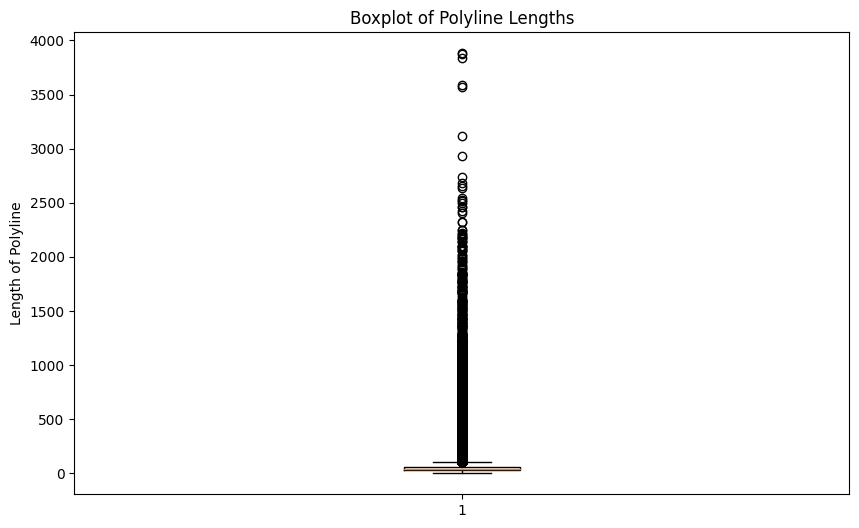
\includegraphics[scale = 0.5]{image/boxplot-length-full.png}
        \caption{Boxplot of the full dataset’s polyline lengths}
        \label{fig:menu}
    \end{figure}
    
    Noticing that these were mostly short, we decided to determine by trial and error a small number of selected points, and this was set at 3 (which is potentially not the optimal solution, but which is, for lack of time, ours).   So, firstly, for polylines of size less than or equal to 2, the first point is repeated 3 times. Then, for polylines of size equal to 3, we retain the first point and repeat the second 2 times. After that, for polylines of size equal to 4, we use the first, second and third points, and finally, for polylines of size greater than 4, we use the first point, the point in the middle of the polyline and a point drawn randomly from the end of the polyline. The destination being chosen for all situations as the last point of the polyline.

    Once we had decided to keep 3 points per polyline, we quickly realized that this could be detrimental to predictions on longer polylines, as the destination of these could be very far from the selected points. This is why we decided to add an outlier management step, which consists in assigning a randomly chosen point in the window located after the last point selected and the last point of the polyline. It's on the basis of the previously generated boxplot, and in particular its maximum non-outlier threshold, that we decide whether such a process is useful or not.
\end{itemize}

\section{Longitude \& latitude analysis}

In order to discover possible outliers, we would have liked to carry out a longitude and latitude analysis of the entire data set, but given the large number of data points, this seemed too time-consuming. We therefore decided to carry out this analysis after reducing the number of points used in the previous step.

\begin{figure}[H]
    \centering
    \begin{subfigure}[t]{.49\textwidth}
        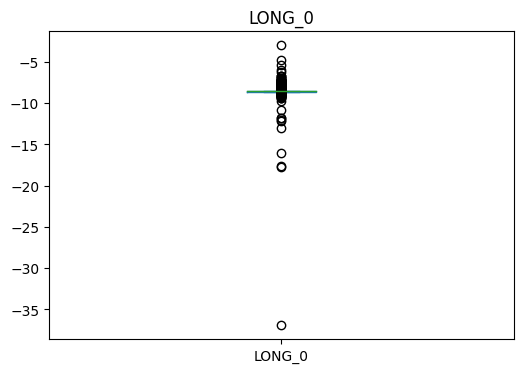
\includegraphics[width =\textwidth]{image/long0_train.png}
        \caption{Longitude of 1st point}
        \label{fig:long_lat}
    \end{subfigure}
    \hfill
    \begin{subfigure}[t]{.49\textwidth}
        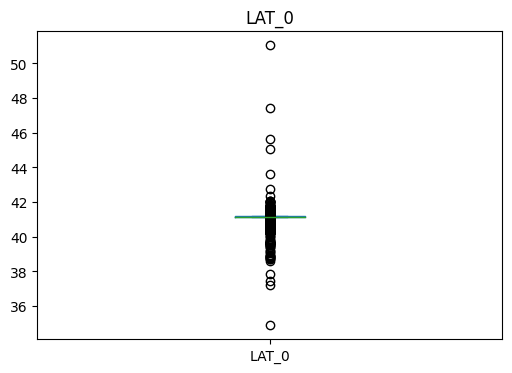
\includegraphics[width =\textwidth]{image/lat0_train.png}
        \caption{Latitude of 1st point}
        \label{fig:long_lat}
    \end{subfigure}
    \hfill
    \begin{subfigure}[t]{.49\textwidth}
        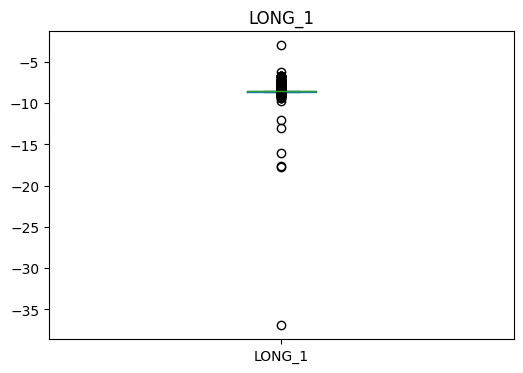
\includegraphics[width =\textwidth]{image/long1_train.png}
        \caption{Longitude of 2nd point}
        \label{fig:long_lat}
    \end{subfigure}
    \hfill
    \begin{subfigure}[t]{.49\textwidth}
        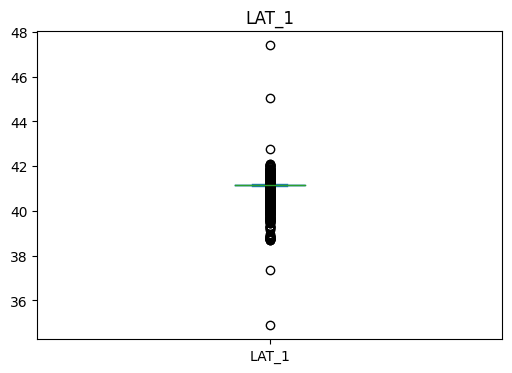
\includegraphics[width =\textwidth]{image/lat1_train.png}
        \caption{Latitude of 2nd point}
        \label{fig:long_lat}
    \end{subfigure}
    \hfill
    \begin{subfigure}[t]{.49\textwidth}
        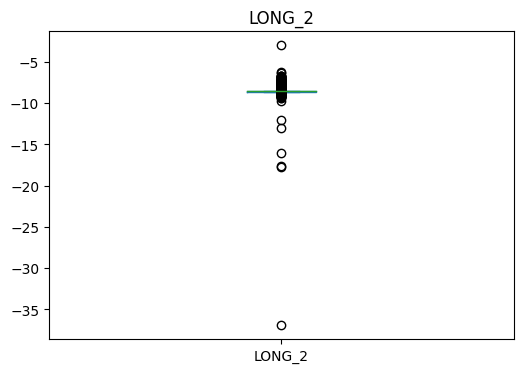
\includegraphics[width =\textwidth]{image/long2_train.png}
        \caption{Longitude of 3rd point}
        \label{fig:long_lat}
    \end{subfigure}
    \hfill
    \begin{subfigure}[t]{.49\textwidth}
        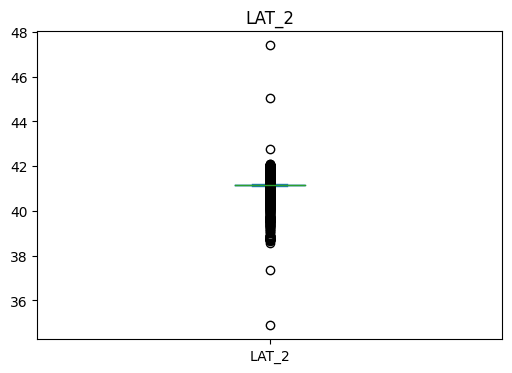
\includegraphics[width =\textwidth]{image/lat2_train.png}
        \caption{Latitude of 3rd point}
        \label{fig:long_lat}
    \end{subfigure}
    \caption{Longitude and latitude of selected points - 75\% of dataset size}
    \label{fig:long_lat}
\end{figure}

\begin{figure}[H]\ContinuedFloat
    \centering
    \begin{subfigure}[t]{.49\textwidth}
        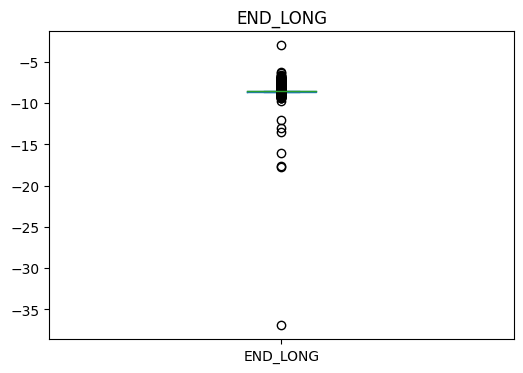
\includegraphics[width =\textwidth]{image/end_long_train.png}
        \caption{Longitude of destination point}
        \label{fig:long_lat}
    \end{subfigure}
    \hfill
    \begin{subfigure}[t]{.49\textwidth}
        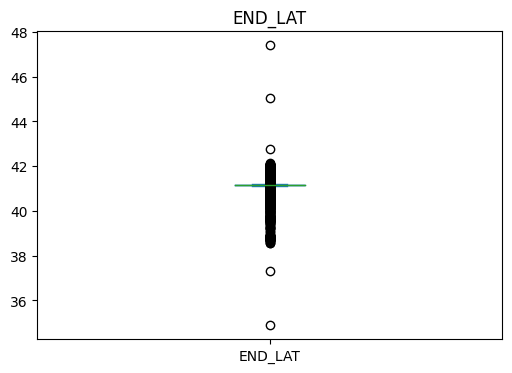
\includegraphics[width =\textwidth]{image/end_lat_train.png}
        \caption{Latitude of destination point}
        \label{fig:long_lat}
    \end{subfigure}
    \caption{Longitude and latitude of selected points - 75\% of dataset size}
    \label{fig:long_lat}
\end{figure}

Once this analysis had been carried out, we hit a dead end: how to deal with these outliers ? One solution might have been to determine a zone around the city of Porto beyond which we would not take the points into account. We would then replace these points with the maximum non-outlier threshold. However, for lack of time and confidence, we preferred to avoid implementing such a process.

\section{Dataset splitting}

Once all this analysis and preprocessing was done, all that remained was to split the dataset into an X and a y on which to train the models. To do this, we simply placed the 3 previously selected points in X and the destination in y.

\section{Model hyperparameters tuning}
Hyperparameters tuning is the technique of choosing the optimal values for the hyperparameters of a machine learning model. They are used to control the behavior of the learning algorithm and can impact on the performance of the model. There are several methods for adjusting hyperparameters. Here are the ones we used:

\subsection{Grid search}

Grid search is an automated method. We simply specify a grid of hyperparameter values to search for, and then each model concerned is trained and evaluated for each combination. The one with the best performance is selected. We used that that approach using 5-fold cross-validation on our dataset for \textit{k-nearest neighbors}, \textit{decision tree} \& \textit{ridge} models.

Grid search, however, has the potential to be computationally costly due to the need to train and assess the model for each combination in the grid. When dealing with huge grids or sophisticated models, this may become impractical. This explains the use of manual tuning as well.

Note that for \textit{kNN}, we were able to use grid search up to 10\% of the dataset size, after which we set its parameters to the last values obtained with grid search.

\subsection{Manual tuning}

Manual tuning involves manually experimenting with various hyperparameter combinations and assessing the model's performance for each one. This technique was used for \textit{random forest} model.

\subsection{Hyperparameter Evolution by Dataset Size}

\begin{table}[ht]
    \centering
    \footnotesize % Set font size to small
    \begin{tabular}{|l|c|c|c|c|c|c|}
        \hline
        \textbf{Algorithm} & \textbf{Dataset Size} & \textbf{Hyperparameter 1} & \textbf{Hyperparameter 2} & \textbf{Hyperparameter 3} \\
        \hline
        \multirow{4}{*}{\textit{K-Nearest Neighbors}} 
        & 0.1\% & 'algorithm': 'auto' & 'n\_neighbors': 512 & 'weights': 'uniform' \\
        & 1\% & 'algorithm': 'auto' & 'n\_neighbors': 128 & 'weights': 'uniform' \\
        & 10\% & 'algorithm': 'auto' & 'n\_neighbors': 256 & 'weights': 'distance' \\
        & 30\% & / & / & / \\
        & 50\% & / & / & / \\
        & 75\% & / & / & / \\
        \hline
        \multirow{4}{*}{\textit{Decision Tree}} 
        & 0.1\% & 'max\_depth': 10 & 'min\_samples\_leaf': 1 & 'min\_samples\_split': 10 \\
        & 1\% & 'max\_depth': 10 & 'min\_samples\_leaf': 1 & 'min\_samples\_split': 2 \\
        & 10\% & 'max\_depth': 10 & 'min\_samples\_leaf': 2 & 'min\_samples\_split': 2 \\
        & 30\% & 'max\_depth': 100 & 'min\_samples\_leaf': 4 & 'min\_samples\_split': 10 \\
        & 50\% & 'max\_depth': 100 & 'min\_samples\_leaf': 4 & 'min\_samples\_split': 10 \\
        & 75\% & 'max\_depth': 1000 & 'min\_samples\_leaf': 4 & 'min\_samples\_split': 2 \\
        \hline
        \multirow{4}{*}{\textit{Ridge}} 
        & 0.1\% & 'alpha': 0.1 & / & / \\
        & 1\% & 'alpha': 0.1 & / & / \\
        & 10\% & 'alpha': 0.1 & / & / \\
        & 30\% & 'alpha': 0.1 & / & / \\
        & 50\% & 'alpha': 0.1 & / & / \\
        & 75\% & 'alpha': 0.1 & / & / \\
        \hline
    \end{tabular}
    \caption{Evolution of Best Hyperparameters per Algorithm as a Function of Dataset Size}
    \label{tab:hyperparameters}
\end{table}


\section{Model analysis}

\begin{figure}[ht]
    \flushleft
    \begin{subtable}{0.4\textwidth}
        \flushleft
        \footnotesize % Set font size to small
        \begin{tabular}{|l|c|c|c|c|c|c|}
            \hline
            & \textbf{KNN} & \textbf{DT} & \textbf{RIDGE} & \textbf{LR} & \textbf{RF} \\
            \hline
            \textit{SCORE} & 3.666 & 3.482 & 3.373 & 3.332 & 3.194 \\
            \hline
        \end{tabular}
        \caption{0.1\% of dataset'size}
        \label{tab:table1}
    \end{subtable}%
    \hspace{2.5cm} % Add horizontal space between the tables
    \begin{subtable}{0.4\textwidth}
        \flushleft
        \footnotesize % Set font size to small
        \begin{tabular}{|l|c|c|c|c|c|c|}
        \hline
        & \textbf{KNN} & \textbf{DT} & \textbf{RIDGE} & \textbf{LR} & \textbf{RF} \\
        \hline
        \textit{SCORE} & 3.669 & 3.177 & 3.202 & 3.195 & 3.021 \\
        \hline
    \end{tabular}
        \caption{1\% of dataset'size}
        \label{tab:table2}
    \end{subtable}
    \hspace{2.5cm}
    \begin{subtable}{0.4\textwidth}
        \flushleft
        \footnotesize % Set font size to small
        \begin{tabular}{|l|c|c|c|c|c|c|}
        \hline
        & \textbf{KNN} & \textbf{DT} & \textbf{RIDGE} & \textbf{LR} & \textbf{RF} \\
        \hline
        \textit{SCORE} & 3.629 & 3.159 & 3.267 & 3.267 & 3.108 \\
        \hline
    \end{tabular}
        \caption{10\% of dataset'size}
        \label{tab:table2}
    \end{subtable}
    \hspace{2.5cm}
    \begin{subtable}{0.4\textwidth}
        \flushleft
        \footnotesize % Set font size to small
        \begin{tabular}{|l|c|c|c|c|c|c|}
        \hline
        & \textbf{KNN} & \textbf{DT} & \textbf{RIDGE} & \textbf{LR} & \textbf{RF} \\
        \hline
        \textit{SCORE} & 3.667 & 3.124 & 3.129 & 3.128 & 3.006 \\
        \hline
    \end{tabular}
        \caption{30\% of dataset'size}
        \label{tab:table2}
    \end{subtable}
    \hspace{2.5cm}
    \begin{subtable}{0.4\textwidth}
        \flushleft
        \footnotesize % Set font size to small
        \begin{tabular}{|l|c|c|c|c|c|c|}
        \hline
        & \textbf{KNN} & \textbf{DT} & \textbf{RIDGE} & \textbf{LR} & \textbf{RF} \\
        \hline
        \textit{SCORE} & 3.661 & 3.072 & 3.227 & 3.227 & 3.044 \\
        \hline
    \end{tabular}
        \caption{50\% of dataset'size}
        \label{tab:table2}
    \end{subtable}
    \hspace{2.5cm}
    \begin{subtable}{0.4\textwidth}
        \flushleft
        \footnotesize % Set font size to small
        \begin{tabular}{|l|c|c|c|c|c|c|}
        \hline
        & \textbf{KNN} & \textbf{DT} & \textbf{RIDGE} & \textbf{LR} & \textbf{RF} \\
        \hline
        \textit{SCORE} & 3.638 & 3.248 & 3.281 & 3.281 & 3.084 \\
        \hline
    \end{tabular}
        \caption{75\% of dataset'size}
        \label{tab:table2}
    \end{subtable}
    \caption{Comparison of measurement for different of dataset'size}
    \label{fig:two-tables}
\end{figure}


As we can in the different Tables \ref{fig:two-tables}, increasing the size of the training dataset can have different effects: 

\begin{itemize}
    \item 
    \textbf{BENEFITS}
    \begin{enumerate}
        \item 
        \textbf{Improved Generalization:}

KNN, Decision Tree, and Random Forest: These algorithms can benefit from a larger dataset as they tend to generalize better with more diverse examples.

\item 
\textbf{Reduced Overfitting:}

Ridge Regression: Increasing the dataset size can help in reducing overfitting, especially when dealing with a large number of features.
\item 
\textbf{Enhanced Model Stability:}

Linear Regression: A larger dataset can lead to a more stable and reliable linear regression model, reducing the impact of outliers.
    \end{enumerate}

    \item 
    \textbf{DRAWBACKS}
    \begin{enumerate}
        \item 
        \textbf{Computational Complexity:}

kNN: The computation of distances in kNN can be computationally expensive with larger datasets, making predictions slower. For example, apply GridSearch on kNN with 30\% of the dataset is taken way too long on Kaggle so we had to tune the parameter of kNN to find the best and then put in the main programm.
        \item 
\textbf{Overfitting Risk:}

Linear Regression: While linear regression models can benefit from more data, there's a risk of overfitting if the model becomes too complex relative to the dataset.
        \item 
\textbf{Tree Depth and Complexity:}

Decision Tree and Random Forest: Increasing the dataset might lead to deeper trees, which can result in overfitting. Proper tuning of hyperparameters is essential.
        \item 
\textbf{Diminishing Returns:}

All Algorithms: There might be a point of diminishing returns, where the additional data provides minimal improvement in model performance.
    \end{enumerate}

    \item 
    \textbf{NOTE} 
    
    As we can see on the different tables, the score become stable after a certain size of dataset for all algorithms so it means that better performance cannot be achieve this way and the improvement has to come from somewhere else like a better preprocessing or scaling the data.
\end{itemize}

\subsection{k-Nearest Neighbors}
K-nearest neighbors (KNN) is a non-parametric approach which bases its predictions on the mean of the target values of the closest K neighbors in the training data. This method is influenced by the scale of the features, often necessitating preprocessing steps for optimal results.

\subsection{Decision Tree}
A particular kind of model called a decision tree bases its predictions on a set of guidelines that it has acquired through training data. It builds a structure like a tree, with each leaf node representing a predicted value for the target variable and each inside node representing a choice based on one of the input features.

\subsection{Ridge}
Ridge regression is a type of linear regression model which incorporates a regularization element into its objective function. This component is designed to constrain the size of the coefficients, aiding in avoiding overfitting. It is particularly useful in situations where there is a high number of predictors and a significant risk of overfitting.

\subsection{Linear Regression}
A popular and straightforward technique for simulating the relationship between a dependent variable and one or more independent variables is linear regression. It uses a least squares method to estimate the coefficients of the model and makes the assumption that the relationship between the variables is linear.

\subsection{Random Forest}
The ensemble technique known as "random forest" aggregates the forecasts from several decision trees. Using bootstrapped samples of the training data, it builds a set of decision trees, each of which predicts the target variable. The average of the predictions each individual tree provided makes up the final forecast.

\subsection{Models that we could not use}

So in our research to find better algorithm to determine the final destination, we have found AdaBoostRegressor and StackingRegressor that are ensemble learning techniques that aim to improve predictive performance by combining the predictions of multiple base models.

For AdaBoost, its strengths are reducing bias and increasing accuracy and being robust to overfitting.
but it is sensitive to noisy data and outliers since we think that we have handled the outliers correctly, it could have some good performance.\\

For Stacking, its strengths is that it can capture complex relationships in the data and utilize the strengths of different models but it requires careful tuning of hyperparameters and is computationally more expensive(which is not really a problem with the power of GPU of the Kaggle notebook).\\

However, due to the disposition of the output (y) in a 2D array and the need of those algorithms to have y in a 1d array they could not be used.


\section{Conclusion \& Improvements}
We chose random forest as the best regression method as by looking at the results, one can see that random forest performs better and gives the best scores. Something we could have done better was to fine tune hyperparameter even more maybe on better preprocessed data.

\end{document}


